\documentclass[a4paper,final]{article}
\usepackage[14pt]{extsizes}
\usepackage[T2A]{fontenc}
\usepackage[utf8]{inputenc}
\usepackage[russian]{babel}




\usepackage{amsmath}
\usepackage[left=20mm, top=20mm, right=20mm, bottom=20mm, footskip=10mm]{geometry}
\usepackage{ragged2e}
\usepackage{setspace}
\usepackage{alltt}
\usepackage{wrapfig}
\usepackage{moreverb} %листинги
\usepackage{indentfirst} % для абзацного отступа
\renewcommand\verbatimtabsize{4\relax}
\renewcommand\listingoffset{0.2em} %отступ от номеров строк
\renewcommand{\arraystretch}{1.4} % высота строки
\usepackage[font=small, singlelinecheck=false, justification=raggedleft, format=plain, labelsep=period]{caption} %заголовок таблицы
\usepackage{listings}
\usepackage{xcolor} % цвета
\usepackage{hyperref}% для гиперссылок
\usepackage{enumitem} %для перечислений
\usepackage{nccmath}
\usepackage{tikz}
\usepackage{wrapfig}
\usepackage{listings}
\usepackage{float}
\usepackage{shadow}
\usepackage{longtable}
\usepackage{multirow}
\usepackage{makecell}
\usepackage{longtable}
\usepackage{tabularx}
\usepackage{seqsplit}
\usepackage{subcaption} % Для подрисунков
\usepackage{tikz}
\usepackage{cmap}
\usetikzlibrary{shapes.geometric, arrows.meta, positioning, calc}
\usepackage{amssymb}
\usepackage{MnSymbol}
\usepackage{wasysym}


\hypersetup{colorlinks,
  allcolors=[RGB]{000 000 000}} %гиперссылки

\textheight=24cm
\textwidth=16cm
\oddsidemargin=0pt
\topmargin=-1.5cm
\parindent=24pt % отступ абзаца по горизонтали
\parskip=5pt % отступ абзаца по вертикали
\tolerance=2000 % терпимость
\flushbottom % выравнивание высоты
\addto\captionsrussian{\def\refname{Список использованной литературы}}
\usepackage{xcolor}

%New colors defined below
\definecolor{codegreen}{rgb}{0,0.6,0}
\definecolor{codegray}{rgb}{0.5,0.5,0.5}
\definecolor{codepurple}{rgb}{0.58,0,0.82}
\definecolor{backcolour}{rgb}{0.95,0.95,0.92}


\definecolor{apricot}{HTML}{FFF0DA}
\definecolor{mygreen}{rgb}{0,0.6,0}
\definecolor{string}{HTML}{B40000} % цвет строк в коде
\definecolor{comment}{HTML}{008000} % цвет комментариев в коде
\definecolor{keyword}{HTML}{1A00FF} % цвет ключевых слов в коде
\definecolor{morecomment}{HTML}{8000FF} % цвет include и других элементов в коде
\definecolor{captiontext}{HTML}{FFFFFF} % цвет текста заголовка в коде
\definecolor{captionbk}{HTML}{999999} % цвет фона заголовка в коде
\definecolor{bk}{HTML}{FFFFFF} % цвет фона в коде
\definecolor{frame}{HTML}{999999} % цвет рамки в коде
\definecolor{brackets}{HTML}{B40000} % цвет скобок в коде

\setlist[enumerate,itemize]{leftmargin=1.2cm}

% подгружаемые языки — подробнее в документации listings
\lstloadlanguages{C++}

\newcommand{\doublecline}[1]{\noalign{\vskip-0.5\arrayrulewidth}\cline{#1}\noalign{\vskip-0.5\arrayrulewidth}\cline{#1}}


\tikzset{
  % Терминал (прямоугольник)
  term/.style={
    rectangle, draw, rounded corners=2pt,
    minimum height=6mm, minimum width=12mm,
    inner sep=3pt, font=\ttfamily\small
  },
  % Нетерминал (угловые скобки, без рамки — курсив)
  nonterm/.style={
    rectangle, draw=none,
    minimum height=6mm,
    inner sep=2pt, font=\itshape\small
  },
  % Ключевое слово (овал — добавлено/изменено, как на оригинале)
  keyword/.style={
    ellipse, draw, fill=white,
    minimum height=6mm, minimum width=14mm,
    inner sep=3pt, font=\ttfamily\small
  },
  % Стрелка линии
  rail/.style={->, >=Stealth, thick},
  % Линия без стрелки
  wire/.style={-, thick},
}


\begin{document}
\lstset{
  inputencoding=utf8,
  language=C++, % Язык кода по умолчанию
  morekeywords={*,...}, % если хотите добавить ключевые слова, то добавляйте
  % Цвета
  keywordstyle=\color{keyword}\ttfamily\bfseries,
  %stringstyle=\color{string}\ttfamily,
  stringstyle=\ttfamily\color{red!50!brown},
  commentstyle=\color{comment}\ttfamily,
  morecomment=[l][\color{morecomment}]{\#},
  % Настройки отображения
  breaklines=true, % Перенос длинных строк
  basicstyle=\ttfamily\footnotesize, % Шрифт для отображения кода
  backgroundcolor=\color{bk}, % Цвет фона кода
  frame=lrb,xleftmargin=\fboxsep,xrightmargin=-\fboxsep, % Рамка, подогнанная к заголовку
  rulecolor=\color{frame}, % Цвет рамки
  tabsize=3, % Размер табуляции в пробелах
  % Настройка отображения номеров строк. Если не нужно, то удалите весь блок
  numbers=left, % Слева отображаются номера строк
  stepnumber=1, % Каждую строку нумеровать
  numbersep=5pt, % Отступ от кода
  numberstyle=\small\color{black}, % Стиль написания номеров строк
  % Для отображения русского языка
  extendedchars=true,
  literate=
  {→}{{\ensuremath{\rightarrow}}}1
  {ε}{{\ensuremath{\varepsilon}}}1
  {á}{{\'a}}1  {é}{{\'e}}1  {í}{{\'i}}1  {ó}{{\'o}}1  {ú}{{\'u}}1
  {Á}{{\'A}}1  {É}{{\'E}}1  {Í}{{\'I}}1  {Ó}{{\'O}}1  {Ú}{{\'U}}1
  {ñ}{{\~n}}1  {Ñ}{{\~N}}1  {¿}{{{\textquestiondown}}}1  {¡}{{{\textexclamdown}}}1
  {Ö}{ {\''O} }1
  {~}{ {\textasciitilde} }1
  {а}{ {\selectfont\char224} }1
  {б}{ {\selectfont\char225} }1
  {в}{ {\selectfont\char226} }1
  {г}{ {\selectfont\char227} }1
  {д}{ {\selectfont\char228} }1
  {е}{ {\selectfont\char229} }1
  {ё}{ {\''e} }1
  {ж}{ {\selectfont\char230} }1
  {з}{ {\selectfont\char231} }1
  {и}{ {\selectfont\char232} }1
  {й}{ {\selectfont\char233} }1
  {к}{ {\selectfont\char234} }1
  {л}{ {\selectfont\char235} }1
  {м}{ {\selectfont\char236} }1
  {н}{ {\selectfont\char237} }1
  {о}{ {\selectfont\char238} }1
  {п}{ {\selectfont\char239} }1
  {р}{ {\selectfont\char240} }1
  {с}{ {\selectfont\char241} }1
  {т}{ {\selectfont\char242} }1
  {у}{ {\selectfont\char243} }1
  {ф}{ {\selectfont\char244} }1
  {х}{ {\selectfont\char245} }1
  {ц}{ {\selectfont\char246} }1
  {ч}{ {\selectfont\char247} }1
  {ш}{ {\selectfont\char248} }1
  {щ}{ {\selectfont\char249} }1
  {ъ}{ {\selectfont\char250} }1
  {ы}{ {\selectfont\char251} }1
  {ь}{ {\selectfont\char252} }1
  {э}{ {\selectfont\char253} }1
  {ю}{ {\selectfont\char254} }1
  {я}{ {\selectfont\char255} }1
  {А}{ {\selectfont\char192} }1
  {Б}{ {\selectfont\char193} }1
  {В}{ {\selectfont\char194} }1
  {Г}{ {\selectfont\char195} }1
  {Д}{ {\selectfont\char196} }1
  {Е}{ {\selectfont\char197} }1
  {Ё}{ {\''E} }1
  {Ж}{ {\selectfont\char198} }1
  {З}{ {\selectfont\char199} }1
  {И}{ {\selectfont\char200} }1
  {Й}{ {\selectfont\char201} }1
  {К}{ {\selectfont\char202} }1
  {Л}{ {\selectfont\char203} }1
  {М}{ {\selectfont\char204} }1
  {Н}{ {\selectfont\char205} }1
  {О}{ {\selectfont\char206} }1
  {П}{ {\selectfont\char207} }1
  {Р}{ {\selectfont\char208} }1
  {С}{ {\selectfont\char209} }1
  {Т}{ {\selectfont\char210} }1
  {У}{ {\selectfont\char211} }1
  {Ф}{ {\selectfont\char212} }1
  {Х}{ {\selectfont\char213} }1
  {Ц}{ {\selectfont\char214} }1
  {Ч}{ {\selectfont\char215} }1
  {Ш}{ {\selectfont\char216} }1
  {Щ}{ {\selectfont\char217} }1
  {Ъ}{ {\selectfont\char218} }1
  {Ы}{ {\selectfont\char219} }1
  {Ь}{ {\selectfont\char220} }1
  {Э}{ {\selectfont\char221} }1
  {Ю}{ {\selectfont\char222} }1
  {Я}{ {\selectfont\char223} }1
  {\{}{ { {\color{brackets}\{} } }1 % Цвет скобок {
  {\} }{ { {\color{brackets}\} } } }1 % Цвет скобок }
}


\thispagestyle{empty}
\begin{center}
\hfill \break
\hfill \break
\normalsize{МИНИСТЕРСТВО НАУКИ И ВЫСШЕГО ОБРАЗОВАНИЯ РОССИЙСКОЙ ФЕДЕРАЦИИ\\
 федеральное государственное автономное образовательное учреждение высшего образования «Санкт-Петербургский политехнический университет Петра Великого»\\[10pt]}
\normalsize{Институт компьютерных наук и кибербезопасности}\\[10pt] 
\normalsize{Высшая школа технологий искусственного интеллекта}\\[10pt] 
\normalsize{Направление: 02.03.01 <<Математика и компьютерные науки>>}\\
\vspace{50pt}
{\large Математическая логика и теория формальных языков\\
Отчёт о выполнении лабораторной работы №5 \\
<<Разработка детерминированного анализатора грамматики LL(1)>>\\[1em]
Вариант 17}
\end{center}
 \vspace{70pt}
\small{ 
\begin{tabular}{lrrl}
\!\!\!Студент, & \hspace{2cm} & & \\
\!\!\!группа 5130201/30102 & \hspace{2cm} & \underline{\hspace{3cm}} & Путята М. А.  \\\\
\!\!\!Преподаватель & \hspace{2cm} & \underline{\hspace{3cm}} &  Востров А. В. \\\\
&&\hspace{5cm}
\end{tabular}
\begin{flushright}
<<\underline{\hspace{1cm}}>>\underline{\hspace{2.5cm}} 2026 г.
\end{flushright}
}

\hfill \break
\begin{center} \small{Санкт-Петербург, 2026} \end{center}


\newpage
\tableofcontents
\newpage

\section*{Введение}
\addcontentsline{toc}{section}{Введение}
В ходе выполнения данной лабораторной работы необходимо провести анализиз заданной грамматики:$$ S \rightarrow aBS ~|~ b,\quad A \rightarrow a, \quad B \rightarrow A ~|~ bSB$$

Для выполнения поставленной задачи необходимо:
\begin{enumerate}
    \item Определить множества FIRST и FOLLOW для каждого нетерминала грамматики.
    \item Построить таблицу выбора.
    \item Построить матрицу отношений предшествования.
    \item Определить тип грамматики.
\end{enumerate}

\newpage
\section{Математическое описание}
\subsection{Контекстно-свободные грамматики}
Контекстно-свободные грамматики относятся являются 2 типом грамматик согласно классификации Хомского. В таких грамматиках продукции имеют вид $A \rightarrow \beta$, где $A$ - нетерминал, а $\beta$ - цепочка, которая может содержать и терминалы и нетерминалы.

Для всех КС-грамматик можно реализовать алгоритм восходящего синтаксического анализа. Восходящий синтаксический анализ заключается в поиске в просматриваемой слева направо сентенциальной форме самой левой связки (подцепочки, совпадающей с правой частью одной из продукций, которая заменяется соответствующим нетерминалом в леовй части). Данный поиск не прекращается до тех пор, пока не будет получен начальный символ грамматики.

\subsection{LL(k)-грамматики}
LL(k)-грамматики - класс грамматик, для которых возможен нисходящий синтаксический анализ, в котором:
\begin{itemize}
    \item входная цепочка просматривается слева направо;
    \item на каждом шаге анализатор может видеть не более чем на k символов вперёд.
\end{itemize}

Для построения LL(k)-грамматик необходимо определить следующие множества:
\begin{itemize}
    \item $\text{FIRST}(\alpha)$ - множество терминальных символов, с которых могут начинаться цепочки, выводимые из $\alpha$. Если $\text{FIRST}(\alpha) ~\cap~ \text{FIRST}(\gamma) = \varnothing$, то можно сделать однозначный выбор между правилами $A \rightarrow \alpha$ и $A \rightarrow \gamma$;
    \item $\text{FOLLOW}(A)$ - множество терминальных цепочек (до k символов), которые могут следовать за $A$ в выводах. Если $\text{FIRST}(\alpha) ~\cap~ \text{FOLLOW}(A) = \varnothing$, можно сделать однозначный выбор между правилами $A \rightarrow \alpha$ и $A \rightarrow \varepsilon$.
\end{itemize}

Формально, в LL(k)-грамматике, если:
\begin{itemize}
    \item $S \rightarrow^* w A\alpha \rightarrow w\beta\alpha \rightarrow^* wx $
    \item $S \rightarrow^* w A\alpha \rightarrow w\gamma\alpha \rightarrow^* wy $
\end{itemize}
где $x, y \in V_T^*$ выполняется условие:$$\text{FIRST}_k(x) = \text{FIRST}_k(y) \rightarrow \beta = \gamma$$

Грамматика является LL(k) тогда и только тогда, когда для каждого нетерминала $A$ и двух любых его продукций $A \rightarrow \alpha$ и $A \rightarrow \beta$ выполняется:$$\text{FIRST}_k(\alpha \text{ FOLLOW}_k(A)) ~\cap~ \text{FIRST}_k(\beta \text{ FOLLOW}_k(A)) \neq \varnothing$$



\subsection{LL(1)-грамматика}
Грамматика является LL(1), если выполняются следующие условия для каждого нетерминала $A$ с продукциями $A \rightarrow \alpha_1 ~|~\alpha_2 ~|~ \dots ~|~ \alpha_n$:
\begin{itemize}
    \item $\forall~ i, j \in \{1, \dots, n\}: i \neq j ~\Rightarrow~\text{FIRST}_1(\alpha_i) ~\cap~ \text{FIRST}_1(\alpha_j) = \varnothing$
    \item $\forall~ i, j \in \{1, \dots, n\}: (i \neq j) \land (\alpha_i \rightarrow^* \varepsilon) ~\Rightarrow~ \text{FIRST}_1(a_j) ~\cap~ \text{FOLLOW}_1(A) = \varnothing $
\end{itemize}

\paragraph{Функции FIRST и FOLLOW для LL(1)}\mbox{}
\begin{itemize}
    \item $\text{FIRST}_1(\alpha) = \{x \in V_T : \alpha \rightarrow^* x\beta\} ~\cup~ \{\varepsilon : \alpha \rightarrow^* \varepsilon\}$
    \item $\text{FOLLOW}_1(A) = \{x \in V_T : S \rightarrow^* \beta A x \gamma\} ~\cup~ \{\$ : S \rightarrow^* \beta A\}$
\end{itemize}

\paragraph{LL(1)-анализатор}\mbox{}

LL(1)-анализатор — это нисходящий детерминированный распознаватель, строящий левый вывод цепочки. При принятии решения он использует текущий нетерминал на вершине стека и один символ текущего входа. Его работа основана на таблице выбора продукций, строки которой соответствуют нетерминалам, а столбцы — терминалам и маркеру конца $\$
$.

Построение таблицы выбора начинается с расширенной грамматики с дополнительным правилом $S' \rightarrow S~\$$ и использует множества FIRST и FOLLOW. Для каждой продукции $A \rightarrow \alpha$ ячейка M[A,t] заполняется следующим образом:
\begin{itemize}
    \item если $t \in \text{FIRST}(\alpha)$, то в $M[A, t]$ записывается $A \rightarrow \alpha$;
    \item если $\varepsilon \in \text{FIRST}(\alpha)$ и $t \in \text{FOLLOW}(A)$, то в $M[A, t]$ также записывается $A \rightarrow \alpha$;
    \item все незаполненные ячейки означают ошибку.
\end{itemize}

\subsection{Заданная грамматика}
Продукции заданной грамматики:
$$S \rightarrow aBS ~|~ b$$ $$A \rightarrow a$$ $$B \rightarrow A ~|~ bSB$$
\subsubsection{Множества FIRST и FOLLOW}
Если для двух альтернатив $A \rightarrow \alpha$ и $A \rightarrow \beta$ множества $\text{FIRST}(\alpha)$ и $\text{FIRST}(\beta)$ не пересекаются, то можно однозначно выбрать нужное правило. Если $\varepsilon \in \text{FIRST}(\alpha)$, то необходимо, чтобы $\text{FOLLOW}(A)$ не пересекалось с $\text{FIRST}(\beta)$ также для однозначного выбора между альтернативами $A \rightarrow \alpha$ и $A \rightarrow \varepsilon$

Вычисление FIRST:
\begin{enumerate}
    \item Для каждого терминала x : $\text{FIRST}(x) = \{x\}$.
    \item Для нетерминалов множества изначально пусты и к ним последовательно добавляются элементы множеств FIRST правых частей правил вывода.
\end{enumerate}

Вычисление FOLLOW:
\begin{enumerate}
    \item в $\text{FOLLOW}(S')$ заносится <<\$>>.
    \item Для каждого правила вывода $A \rightarrow \alpha B \beta$ в $\text{FOLLOW}(B)$ добавляются элементы из $\text{FIRST}(\beta)$. Если цепочка $\beta$ может быть пустой, то также добавляется $\text{FOLLOW}(A)$.
\end{enumerate}

Построение множеств FIRST:
\begin{itemize}
    \item $\text{FIRST}(a)$ = \{a\};
    \item $\text{FIRST}(b)$ = \{b\};
    \item $\text{FIRST}(S)$ = $\text{FIRST}(aBS) ~\cup~ \text{FIRST}(b)$ = $\{a\} ~\cup \{b\}~$ = $\{a, b\}$;
    \item $\text{FIRST}(S')$ = $\text{FIRST}(S\$)$ = $\text{FIRST}(S)$ = $\{a, b\}$;
    \item $\text{FIRST}(A)$ = $\text{FIRST}(a)$ = $\{a\}$;
    \item $\text{FIRST}(B)$ = $\text{FIRST}(A) ~\cup~ \text{FIRST}(bSB)$ = $\{a\} ~\cup~ \{b\}$ = $\{a, b\}$
\end{itemize}

Построение множеств FOLLOW:
\begin{itemize}
    \item $\text{FOLLOW}(S') = \{\$\}$
    \item $\text{FOLLOW}(S) \supset \{\$\}$ (из $S' \rightarrow S~\$$)
    \item $\text{FOLLOW}(S) \supset \text{FIRST}(B) = \{a, b\}$ (из $B \rightarrow bSB$)
    \item $\text{FOLLOW}(B) \supset \text{FIRST}(S) = \{a, b\}$ (из $S \rightarrow aBS$)
    \item $\text{FOLLOW}(A) \supset \text{FOLLOW}(B) = \{a, b\}$ (из $B \rightarrow A$)
\end{itemize}

В таблицах 1 представлены множества FIRST и FOLLOW для заданной грамматики.


\begin{table}[H]
    \centering
    \caption{\centering Множества FIRST и FOLLOW}
    \begin{tabular}{|c|c|c|}\hline
        Нетерминал & FIRST & FOLLOW\\\hline
        S' & \{a, b\} & \{\$\}\\
        S & \{a, b\} & \{a, b, \$\}\\
        A & \{a\} & \{a, b\}\\
        B & \{a, b\} & \{a, b\}\\\hline
    \end{tabular}
\end{table}

\subsubsection{Проверка условия LL(1)}
Грамматика будет являться LL(1), если для любых двух альтернатив одного нетерминала $A \rightarrow \alpha$ и $A \rightarrow \beta$ выполняется $\text{FIRST}(\alpha) ~\cap~ \text{FIRST}(\beta) = \varnothing$. Условие $\varepsilon \in \text{FIRST}(\alpha) \Rightarrow \text{FIRST}(\beta) ~\cap~ \text{FOLLOW}(A) = \varnothing$ проверяться не будет, так как в продукциях грамматики отсутствует $\varepsilon$.

\begin{itemize}
    \item \textbf{Проверка для S}: $\text{FIRST}(aBS) ~\cap~ \text{FIRST}(b) = \{a\} ~\cap~ \{b\} = \varnothing$;
    \item \textbf{Проверка для B}: $\text{FIRST}(A) ~\cap~ \text{FIRST}(bSB) = \{a\} ~\cap~ \{b\} = \varnothing$;
    \item Нетерминал $A$ имеет одну продукцию - конфликтов нет;
\end{itemize}

Конфликты не найдены, следовательно грамматика является LL(1).

\subsubsection{Таблица выбора}

На основе вычисленных множеств FIRST и FOLLOW была построена таблица выбора, на которой отображены соответствующие продукции и выводы ошибок. Таблица выбора представлена в таблице 2.


\begin{table}[H]
    \centering
    \caption{\centeringтаблица выбора}
    \begin{tabular}{|c|c|c|c|}\hline
        Нетерминал & a & b & \$\\\hline
        $S'$ & $S' \rightarrow S~\$$ & $S' \rightarrow S~\$$ & Ошибка\\
        $S$ & $S \rightarrow aBS$ & $S \rightarrow b$ & Ошибка\\
        $A$ & $A \rightarrow a$ & Ошибка & Ошибка\\
        $B$ & $B \rightarrow A$ & $B \rightarrow bSB$ & Ошибка\\\hline
    \end{tabular}
\end{table}

\subsubsection{Грамматика простого предшествования}
Метод отношений предшествования позволяет выделить связку, анализируя отношения между парами соседних символов сентенциальной формы. Вводятся три бинарных отношения:
\begin{itemize}
    \item $X \lessdot Y$ - символ X может находиться непосредственно перед левой границей связки, содержащей Y;
    \item $X \eqdot Y$ - оба символа находятся внутри одной связки;
    \item $X \gtrdot Y$ - символ X может находится непосредственно перед правой границей связки, содержащей Y.
\end{itemize}

Отношения определяются следующими правилами:
\begin{itemize}
    \item $X \eqdot Y \Longleftrightarrow \exists A \rightarrow \alpha X Y\beta \in R$;
    \item $X \lessdot Y \Longleftrightarrow \exists A \rightarrow \alpha X M \beta \in R, ~~M \rightarrow^+ Y\gamma$
\item $X \gtrdot Y \Longleftrightarrow \exists A \rightarrow \alpha M Z \beta \in R, ~~M \rightarrow^+ \gamma X, ~~Z\rightarrow^* Y\delta, ~~ Y \in T$.
\end{itemize}

Грамматика простого предшествования - грамматика, для которой выполняется следующее:
\begin{itemize}
    \item матрица данных отношений не содержит $\varepsilon$-продукций;
    \item матрица данных отношений содержит не более одного отношения на пару символов;
    \item все правые части различны.
\end{itemize}

Анализ выполняется при помощи стека: связкой считается самая левая подстрока, ограниченная слева символом "$\lessdot$" и справа символом "$\gtrdot$", а внутри содержащая только "$\eqdot$". После нахождения связка сворачивается к соответствующему нетерминалу, и процесс продолжается.

\paragraph{Способы нахождения данных отношений}\mbox{}

\textbf{Отношение одновременной сворачиваемости $\eqdot$}
\begin{enumerate}
    \item Двa символа Х и Y могут иметь отношение одновременной сворачиваемости ($X \eqdot Y$), если существует правая часть какой-либо продукции грамматики, в которой эти два символа стоят рядом.
\end{enumerate}

\textbf{Отношение сворачиваемости $\lessdot$}
\begin{enumerate}
    \item Находим в правилах все пары рядом стоящих <символ> <нетерминал>.
    \item <символ> будет находиться в отношении $\lessdot$ со всеми символами, с которых начинаются цепочки, выводимые из <нетерминала>.
\end{enumerate}

\textbf{Отношение сворачиваемости $\gtrdot$}
\begin{enumerate}
    \item Находим в правилах все пары рядом стоящих <нетерминал> <символ>.
    \item Все символы, которыми кончаются цепочки, выводимые из <нетерминала>, будут находиться в отношении $\gtrdot$ с теми терминалами, с которых начинаются цепочки, выводимые из <символа>.
\end{enumerate}

\subsubsection{Матрица отношений простого предшествования}

Заменим продукцию $S' \rightarrow S ~\$$ на $S' \rightarrow \#~S~\#$.

\begin{itemize}
    \item \textbf{Отношения "$\eqdot$"}. Пары: \#S, S\#, aB, BS, bS, SB.
    \item \textbf{Отношения "$\lessdot$"}. Пары: \#S, aB, BS, bS, SB.\\ Отсюда следует: \{\#, B, b\} $\lessdot$ \{a, b\} и \{a, S\} $\lessdot$ \{a, b, A\}
    \item \textbf{Отношения "$\gtrdot$"}. Пары: S\#, BS, SB.\\ Отсюда следует: \{S, b\} $\gtrdot$ \{\#, B, A, a\} и \{B, A, a\} $\gtrdot$ \{a, b\}
\end{itemize}

Для грамматики была построена матрица отношений простого предшествования. В полученной матрице наблюдается много ячеек, в которых находится несколько символов сразу, что указывает на наличие конфликтов. Матрица предшествования представлена в таблице 3.

\begin{table}[H]
    \centering
    \caption{\centeringМатрица предшествования}
    \begin{tabular}{|c|c|c|c|c|c|c|}\hline
         & \# & S & A & B & a & b\\\hline
        \# &  & $\eqdot$ &  &  & $\lessdot$ & $\lessdot$ \\\hline
        S & $\eqdot$ $\gtrdot$ &  & $\lessdot$ $\gtrdot$ & $\eqdot$ $\gtrdot$ & $\lessdot$ $\gtrdot$ & $\lessdot$ \\\hline
        A &  & $\gtrdot$ &  &  & $\gtrdot$ & $\gtrdot$ \\\hline
        B &  & $\eqdot$ $\gtrdot$ &  &  & $\lessdot$ $\gtrdot$ & $\lessdot$ $\gtrdot$ \\\hline
        a &  & $\gtrdot$ &  $\lessdot$ & $\eqdot$ & $\lessdot$ $\gtrdot$ & $\lessdot$ $\gtrdot$ \\\hline
        b & $\gtrdot$ & $\eqdot$ & $\gtrdot$ & $\gtrdot$ & $\lessdot$ $\gtrdot$ & $\lessdot$ \\\hline
    \end{tabular}
\end{table}

Конфликт $S \eqdot \#$ и $S \gtrdot \#$ объясняется тем, что:
\begin{itemize}
    \item в правой части правила <<$S' \rightarrow \#S\#$>> присутствует <<$S\#$>>;
    \item из нетерминала $S$ выводится цепочка оканчивающаяся символом <<$S$>>, а символ \# начинается с терминала \#.
\end{itemize}

\subsection{LL(1)-автомат}

LL(1)-анализ выполняется при помощи стекового автомата, управляемого
таблицей выбора. В начальный момент в стек помещается маркер конца
входа~\$ и начальный символ~$S'$ (на вершине стека).

На каждом шаге анализатор сравнивает вершину стека~$X$ с текущим
символом входа~$a$:

\begin{itemize}
    \item если $X = a$ --- терминал совпадает с текущим символом входа:
    снять $X$ со стека и перейти к следующему символу входа;

    \item если $X = \$$ и $a = \$$ --- цепочка принята (accept);

    \item если $X$ --- нетерминал: обратиться к ячейке $M[X,\, a]$
    таблицы выбора; если продукция $X \to \alpha$ найдена, заменить
    $X$ на вершине стека цепочкой $\alpha$, помещая символы в обратном
    порядке (крайний левый символ оказывается на вершине); если ячейка
    пуста --- зафиксировать ошибку и остановить разбор.
\end{itemize}

Построенная для расширенной грамматики с дополнительным правилом
$S' \to S\$$ таблица выбора содержит 4~строки
и 3~столбца, как показано
в таблице 2.

Работа автомата на примере цепочки $aab$ представлена
в таблице 4.

\begin{table}[h]
\centering
\caption{\centeringРабота LL(1)-анализатора для цепочки $aab$}
\begin{tabular}{|c|l|l|l|}
\hline
\textbf{Шаг} & \textbf{Стек} & \textbf{Вход} & \textbf{Действие} \\
\hline
1  & $S'\,\$$                  & $aab\$$  & $S' \to S\$$       \\
\hline
2  & $S\,\$\,\$$               & $aab\$$  & $S \to aBS$        \\
\hline
3  & $a\,B\,S\,\$\,\$$         & $aab\$$  & совпадение $a$     \\
\hline
4  & $B\,S\,\$\,\$$            & $ab\$$   & $B \to A$          \\
\hline
5  & $A\,S\,\$\,\$$            & $ab\$$   & $A \to a$          \\
\hline
6  & $a\,S\,\$\,\$$            & $ab\$$   & совпадение $a$     \\
\hline
7  & $S\,\$\,\$$               & $b\$$    & $S \to b$          \\
\hline
8  & $b\,\$\,\$$               & $b\$$    & совпадение $b$     \\
\hline
9  & $\$\,\$$                  & $\$$     & совпадение \$      \\
\hline
10 & $\$$                      & $\$$     & accept             \\
\hline
\end{tabular}
\end{table}


\subsubsection{Примеры вывода дерева цепочки}
\begin{figure}[H]
    \centering
    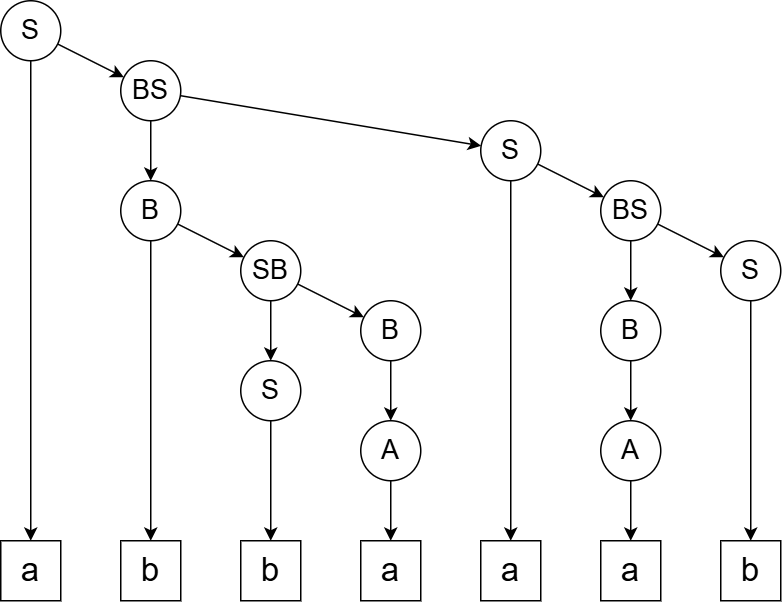
\includegraphics[width=0.6\linewidth]{дерево лаб5.png}
    \caption{\centeringПример вывода дерева цепочки №1}
\end{figure}

\begin{figure}[H]
    \centering
    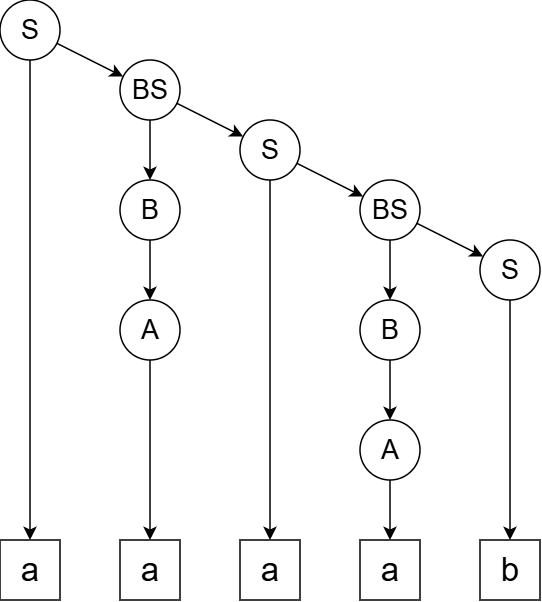
\includegraphics[width=0.5\linewidth]{Дерево лаб 5 2.png}
    \caption{\centeringПример вывода дерева цепочки №2}
\end{figure}

\subsection{Семантические действия}

В работе реализована музыкальная интерпретация: терминал $a$ содержит
строку «\twonotes», терминал $b$ — «\quarternote».

Для каждой продукции задано собственное семантическое действие,
генерирующее текстовое описание музыкальной фразы путём конкатенации
значений, как показано в таблице~\ref{tab:sem}.

\begin{table}[h]
\centering
\caption{Семантические действия продукций}
\label{tab:sem}
\begin{tabular}{|c|c|}
\hline
\textbf{Продукция} & \textbf{Семантическое действие} \\
\hline
$S' \to S$   & вернуть $S$ \\
\hline
$S \to aBS$  & вернуть $a + B + S$ \\
\hline
$S \to b$    & вернуть $b$ \\
\hline
$A \to a$    & вернуть $a$ \\
\hline
$B \to A$    & вернуть $A$ \\
\hline
$B \to bSB$  & вернуть $b + S + B$ \\
\hline
\end{tabular}
\end{table}

Таким образом, результатом разбора цепочки является строка,
представляющая собой конкатенацию музыкальных элементов в порядке
их появления в выводе. Например, цепочка $aab$ порождает строку
«\twonotes \twonotes \quarternote», а цепочка $b$ — строку «\quarternote».

\newpage
\section*{Заключение}
В ходе выполнения лабораторной работы был проведён анализ контекстно-свободной грамматики:

$S \rightarrow aBS ~|~ b,\quad A \rightarrow a,\quad B \rightarrow A ~|~ bSB$

Для каждого нетерминала были вычислены множества FIRST и FOLLOW. Проверка условия LL(1) показала, что для всех нетерминалов с несколькими альтернативами множества FIRST попарно не пересекаются: для S — $\text{FIRST}(aBS) ~\cap~ \text{FIRST}(b) = {a} \cap {b} = \varnothing$, для B — $\text{FIRST}(A) ~\cap~ \text{FIRST}(bSB) = {a} \cap {b} = \varnothing$.

Также была построена матрица отношений простого предшествования с целью проверки принадлежности грамматики этому классу. Однако в полученной матрице были обнаружены конфликты: многие пары содержат одновременно несколько отношений, что нарушает требование наличия не более одного отношения на каждую пару символов. Следовательно, грамматика не является грамматикой простого предшествования.

В рассматриваемой грамматике не была найдена левая рекурсия, но были найдены правые рекурсии. После анализа заданной грамматики, можно сделать вывод, что данная грамматика является LL(1)-грамматикой, которая допускает нисходящий синтаксический анализ.

\paragraph{Масштабирование}\mbox{}
\begin{itemize}
    \item создать программную реализацию данной грамматики.
\end{itemize}

\newpage
\addcontentsline{toc}{section}{Список использованной литературы}
\begin{thebibliography}{}
    \bibitem{litlink1} Секция <<Телематика>>.— Текст: электронный // tema.spbstu: [сайт].— URL: https://tema.spbstu.ru/mathem/ (дата обращения: 21.05.2026).
\end{thebibliography}

% =============================================================
% Этот код вставить в пункт 2e) ПОСЛЕ раздела "Результаты вычислений"
% и ПЕРЕД строкой "Вывод: sqrt(n) D_n = 3.222 > ..."
% =============================================================

% --- Таблица первых 10 строк ---
\begin{table}[H]
\centering
\caption{Первые 10 строк таблицы вычисления статистики Колмогорова}
\begin{tabular}{|c|r|r|r|r|r|r|r|}
\hline
$i$ & $X_{(i)}$ & $\dfrac{i-1}{n}$ & $\dfrac{i}{n}$ & $F_0(X_{(i)})$ &
$\left|F_0 - \dfrac{i-1}{n}\right|$ & $\left|F_0 - \dfrac{i}{n}\right|$ & max\\
\hline
1  & $-1.493$ & 0.0000 & 0.0200 & 0.0861 & 0.0861 & 0.0661 & 0.0861\\
2  & $-1.348$ & 0.0200 & 0.0400 & 0.2611 & 0.2411 & 0.2211 & 0.2411\\
3  & $-1.287$ & 0.0400 & 0.0600 & 0.3688 & 0.3288 & 0.3088 & 0.3288\\
4  & $-1.266$ & 0.0600 & 0.0800 & 0.4090 & 0.3490 & 0.3290 & 0.3490\\
5  & $-1.220$ & 0.0800 & 0.1000 & 0.5000 & 0.4200 & 0.4000 & 0.4200\\
6  & $-1.192$ & 0.1000 & 0.1200 & 0.5557 & \textbf{0.4557} & 0.4357 & \textbf{0.4557}\\
7  & $-1.189$ & 0.1200 & 0.1400 & 0.5616 & 0.4416 & 0.4216 & 0.4416\\
8  & $-1.185$ & 0.1400 & 0.1600 & 0.5695 & 0.4295 & 0.4095 & 0.4295\\
9  & $-1.167$ & 0.1600 & 0.1800 & 0.6045 & 0.4445 & 0.4245 & 0.4445\\
10 & $-1.158$ & 0.1800 & 0.2000 & 0.6217 & 0.4417 & 0.4217 & 0.4417\\
\hline
\end{tabular}
\end{table}

% --- Таблица строки с максимумом ---
\begin{table}[H]
\centering
\caption{Строка с максимальным значением статистики Колмогорова}
\begin{tabular}{|c|r|r|r|r|r|r|r|}
\hline
$i$ & $X_{(i)}$ & $\dfrac{i-1}{n}$ & $\dfrac{i}{n}$ & $F_0(X_{(i)})$ &
$\left|F_0 - \dfrac{i-1}{n}\right|$ & $\left|F_0 - \dfrac{i}{n}\right|$ & max\\
\hline
6 & $-1.192$ & 0.1000 & 0.1200 & 0.5557 & \textbf{0.4557} & 0.4357 & \textbf{0.4557}\\
\hline
\end{tabular}
\end{table}

\end{document}